%%%%%%%%%%%%%%%%%%%% author.tex %%%%%%%%%%%%%%%%%%%%%%%%%%%%%%%%%%%
%
% sample root file for your "contribution" to a contributed volume
%
% Use this file as a template for your own input.
%
%%%%%%%%%%%%%%%% Springer %%%%%%%%%%%%%%%%%%%%%%%%%%%%%%%%%%%%%%%%%


%% RECOMMENDED %%%%%%%%%%%%%%%%%%%%%%%%%%%%%%%%%%%%%%%%%%%%%%%%%%%
%\documentclass[graybox]{svmult}
%
%% choose options for [] as required from the list
%% in the Reference Guide
%
%\usepackage{mathptmx}       % selects Times Roman as basic font
%\usepackage{helvet}         % selects Helvetica as sans-serif font
%\usepackage{courier}        % selects Courier as typewriter font
%\usepackage{type1cm}        % activate if the above 3 fonts are
                             % not available on your system
%
%\usepackage{makeidx}         % allows index generation
%\usepackage{graphicx}        % standard LaTeX graphics tool
%                             % when including figure files
%\usepackage{multicol}        % used for the two-column index
%\usepackage[bottom]{footmisc}% places footnotes at page bottom
%
%% see the list of further useful packages
%% in the Reference Guide
%
%\makeindex             % used for the subject index
%                       % please use the style svind.ist with
%                       % your makeindex program
%
%%%%%%%%%%%%%%%%%%%%%%%%%%%%%%%%%%%%%%%%%%%%%%%%%%%%%%%%%%%%%%%%%%%%%%%%%%%%%%%%%%%%%%%%%%
%
%\begin{document}

\title{Transportation Networks}
% Use \titlerunning{Short Title} for an abbreviated version of
% your contribution title if the original one is too long
\author{
    \textbf{Adam Zsarnóczay}
    \and Jack W. Baker
    \and Rodrigo Silva-Lopez
    \and Ertugrul Taciroglu}
\tocauthor{}
\authorrunning{Zsarnóczay et al.}
% Use \authorrunning{Short Title} for an abbreviated version of
% your contribution title if the original one is too long
%\institute{Name of First Author \at Name, Address of Institute, %\email{name@email.address}
%\and Name of Second Author \at Name, Address of Institute %\email{name@email.address}}
%
% Use the package "url.sty" to avoid
% problems with special characters
% used in your e-mail or web address
%
\maketitle

Transportation systems play an important role in regional response and recovery after a disaster. Roads, railways, and bridges and the interdependencies between these systems and other parts of the built environment shall be considered in comprehensive regional risk assessments. There are several challenges in the performance assessment of transportation networks, from the realistic representation of spatially correlated Intensity Measures (IMs), through collecting exposure data that describes the location, geometric, material, and design characteristics of the network components, to developing models for their response and damage estimation. Finally, the consequences of network damage are measured by evaluating the quality of service (e.g., travel times, trips made). These calculations introduce a set of additional challenges. Computing travel delays requires modeling the behavior of people which is highly nonlinear and difficult to predict in a reliable manner in lieu of post-disaster travel data.
 
\section{Input and Output Data}
\label{sec:perf_transport_io}

Performance of the transportation infrastructure requires inputs and provides outputs at a regional scale. Conceptually, some of the inputs are similar to those required for building performance assessment, but the regional analysis introduces additional challenges such as the necessity to consider spatial correlation in hazard severity and the significant increase in computational complexity of consequence estimation due to the need to model traffic on the damaged network. The following list focuses on the differences and the additional details required when compared to building performance assessment.
% \newline

\paragraph{Hazard characterization} Regardless of the type of hazard considered, its severity needs to be described by one ore more two-dimensional IM fields. Each field represents one hazard scenario and prescribes an IM map for the region. In earthquake engineering, these IMs are typically derived from probabilistic analyses and researchers need to model the correlation between different locations and different IMs to ensure that the IM fields provide a realistic representation of a ground motion scenario \citep[e.g.,][]{lee2006uncertainty, han2012probabilistic, loth2013spatial}. The probabilistic description of wind and water flow characteristics under a hurricane or tsunami are considerably more challenging and not part of the typical research workflow. Non-seismic hazards are often investigated based on scenario events and the IM field under each scenario is a result of a separate, physics-based hazard simulation (REF-HurricaneTranspScenario]). These IM fields represent realistic scenarios; the challenge in this case is to efficiently capture the range of possible IMs with a finite number of hazard simulations. 

\paragraph{Engineering demand parameters} Road and railroad track damage is usually estimated using fragility functions that link intensity measures directly to damage states (e.g., relationships between ground deformation and road damage (REF-RoadFragilityFunction)). In such cases, because performance assessment of these network components does not involve explicit simulation of the roadway (or railroad) components, it does not involve calculation of EDPs. Exceptions to this may include cases where empirical relationships do not apply (e.g., roadways along natural or engineered embankments (REF-SpecialRoadFragility)) or to critical infrastructure (e.g., high-speed rail tracks (REF-HighSpeedRailFragility)).

Bridge damage can be estimated directly from intensity measures \citep[e.g.,][]{fema2018earthquaketechnical}, but the high-fidelity performance assessment of bridges typically involves structural simulation to relate specific EDPs to critical damage states in structural components. Depending on the component these are local deformations, internal forces, or a DM derived from these quantities \citep[e.g.,][]{park1985mechanistic} that are well-correlated with the damage states of the particular component \citep{choi2004seismic}. Estimation of these EDPs with sufficient accuracy requires nonlinear response history analysis on reliable models; hence the computational resources available are an important factor when deciding the level of modeling fidelity.

\paragraph{Fragility functions} These functions describe the probability of exceeding a particular DS of the network component given either an EDP that describes component response (e.g., REF-BridgeEDPFragility) or an IM that describes the severity of the hazard at the site (e.g., REF-BridgeIMFragility). Both approaches are based on laboratory tests and past experience in post-disaster inspection. Conceptually, they are similar to building fragility functions.
% \newline

\paragraph{Consequence functions} The likelihood of direct loss of life and injury due to transportation network damage is significantly lower than the likelihood of such events due to building damage. Hence, studies focus more on estimating the cost of reconstruction and downtime for each component as a function of the damage severity expressed by the DS \citep{stergiou2006treatment} (REF-BridgeRecovery). Losses estimated at the component level directly from component damages cannot consider system-level effects and interdependencies. These consequence functions need to be complemented with a system-level analysis of indirect consequences.

\paragraph{Traffic models} Network performance assessment and evaluation of the consequences of network component damage at a regional scale require a model of traffic flow with source and destination data. Development of a traffic model for a large urban area is a large undertaking. Such models are prepared and used by local transport authorities, and are typically not publicly available. There are good examples of collaboration between academia and local authorities that allow researchers to take advantage of the mature models and vast data available at the authorities (REF-TrafficModel).

\paragraph{Decision variables} Transportation network performance is described by systemwide downtime, the change in traffic, or the change in network capacity given the traffic model described above. Probabilistic assessment of network performance requires a complex and computationally demanding analysis. Performance metrics that shall serve as decision variables are a topic of ongoing research (Miller and Baker, 2016, Miller-Hooks, 2012). Changes in travel time (either regional statistics or focusing on a particular route) and accessibility are two commonly used metrics.

\section{Modeling Approaches}
\label{sec:perf_transport_methods}

Natural disaster impact on a transportation network uses the assumption of independent calculation steps from building performance assessment \citep{Change et al., 2000, kiremidjian2006pacific, Miller and Baker, 2016}. Hence, the hazard characterization, response estimation, damage estimation, and consequence estimation are performed by independent stochastic models. This allows for the following approach to regional simulation (Figure \ref{fig:perf_TranspFramework}):

\begin{itemize}
    \item characterize the hazard in the region using a IM fields;
    \item estimate the response and the corresponding damage in each network component given the IM at the location of the component;
    \item estimate the downtime and repair cost for each network component and assess the performance of the transportation network given the level of damage in network components.
\end{itemize}

\begin{figure}[htb]
    \centering
    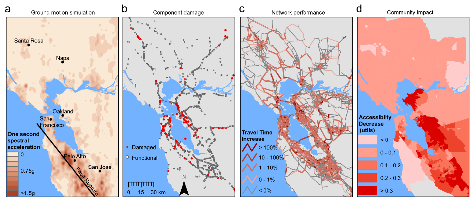
\includegraphics[width=1.0\textwidth, angle = 0]{Figures/RiskAssessmentFramework.pdf}
    \caption{Illustration of the transportation network risk assessment framework from Miller and Baker \cite{miller2015estimating}}
    \label{fig:perf_TranspFramework}
\end{figure}

Structural response and damage (but not the consequences) in one network component is typically assumed to be independent of other components. This assumption enables more efficient simulation through parallel calculation of component damage in the region. It is expedient to note that this approach may overlook correlations in certain bridges that are designed and detailed in similar ways (e.g., bridges along major highways that may have been designed and constructed under one project). The spatially correlated IMs still ensure that similar components within a small area will experience similar demands and, consequently, similar damages.

If sufficiently detailed information of the transportation network is available, the cascading failure of components can be considered; for example, if one overpass fails, its collapse triggers the collapse of others in a complex highway interchange. Consideration of this type of interaction between network components prohibits independent, parallel assessment of network component damage.

A special but important case of transportation network analysis is the investigation of flood risk to the underground transport infrastructure. Such risk can be evaluated by computing the volume of water entering the tunnels based on the time history of flood height at each opening. The performance of the underground system can be evaluated based on the degree of flooding in each of its tunnels. This methodology is available in the GIS-based analysis tool of \cite{jacob2011responding}.

\section{Software and Systems}
\label{sec:perf_transport_tools}

The software that helps with characterization of the hazard and estimation of network component response were introduced in Chapters 1 and 2, respectively. Some of the following tools have such capabilities, but the focus here is on the performance-assessment-related features.

\paragraph{HAZUS 4.2} This FEMA-supported tool has been introduced in Section 1.1. The \citeprgm{HAZUS4x2} Multi-hazard Loss Estimation Methodology provides a comprehensive framework, fragility, and consequence functions for seismic damage and reconstruction time assessment for bridges and transportation links. It also provides a model for assessment of bridge damage due to storm surge. HAZUS cover large groups of bridges with a single configuration. Hence, the damage and recovery estimates cannot account for detailed information about structure type and geometry or the site-specific post-disaster conditions. Evaluation of the impact of component damage on network performance requires external tools.

\paragraph{OpenQuake} The risk assessment framework of the \citeprgm{OpenQuake} tool (introduced in Section 3.1) is sufficiently flexible to enable the assessment of damage and consequences for transportation network components. Unlike HAZUS, the fragility and consequence information is not provided with the tool. The functions available in the HAZUS technical manual \citep{division2018hazusa} can be adopted with minor effort.

\section{Research Gaps and Needs}
\label{sec:perf_transport_gaps}

The regional assessment methodology for transportation networks in HAZUS 4.2 is known to have critical shortcomings \citep[e.g.][]{mangalathu2017bridge}. State-of-the-art transportation network analyses need to develop tools to construct robust bridge models and integrate the regional damage simulations with state-of-the-art traffic and socio-economic impact analyses. These bridge models should be shared with the broader research community so that bridge inventories at regional scales can be compiled and analyzed. Such a capability stands to revolutionize seismic resilience assessment studies and could be extended to other hazards (e.g., tsunamis and hurricanes). Efforts in the aforementioned directions are relatively sparse at the present time (see, for example, \citep{koc2020comprehensive}), but they stand to provide a natural interface between engineers, researchers, as well as practitioners, including insurance agencies/companies, emergency response managers/planners, traffic engineers, and social scientists. 

The following areas appear ripe for directing and supporting research efforts:
\begin{itemize}
    \item Development of tools to generate large inventories of bridge models that can improve upon as more data is available and shared with other members of the natural hazard engineering community. These efforts will likely feature computer vision, machine learning, and data-harvesting techniques.
    \item Studies on devising system-level hazard resilience metrics that take into account the inherent dependency of the subject infrastructure (e.g., port facilities) to regional transportation network performance
    \item Development of workflows and tools to facilitate regional-scale risk and loss assessment studies involving transportation networks
    \item Development of new tools to accurately estimate bridge downtimes and the resulting effects on mobility
\end{itemize}

